\documentclass{article}

\usepackage{graphicx}
\usepackage{tikz}
\usepackage{tikzsymbols}
\usetikzlibrary{calc,patterns,shapes.geometric}
\pagestyle{empty}
\usepackage[margin=0pt]{geometry}
\geometry{papersize={14in,12in}}

\def\centerarc[#1](#2)(#3:#4:#5){\draw[#1] ($(#2)+({#5*cos(#3)},{#5*sin(#3)})$) arc (#3:#4:#5);}

\begin{document}
	\begin{figure}
		\centering
		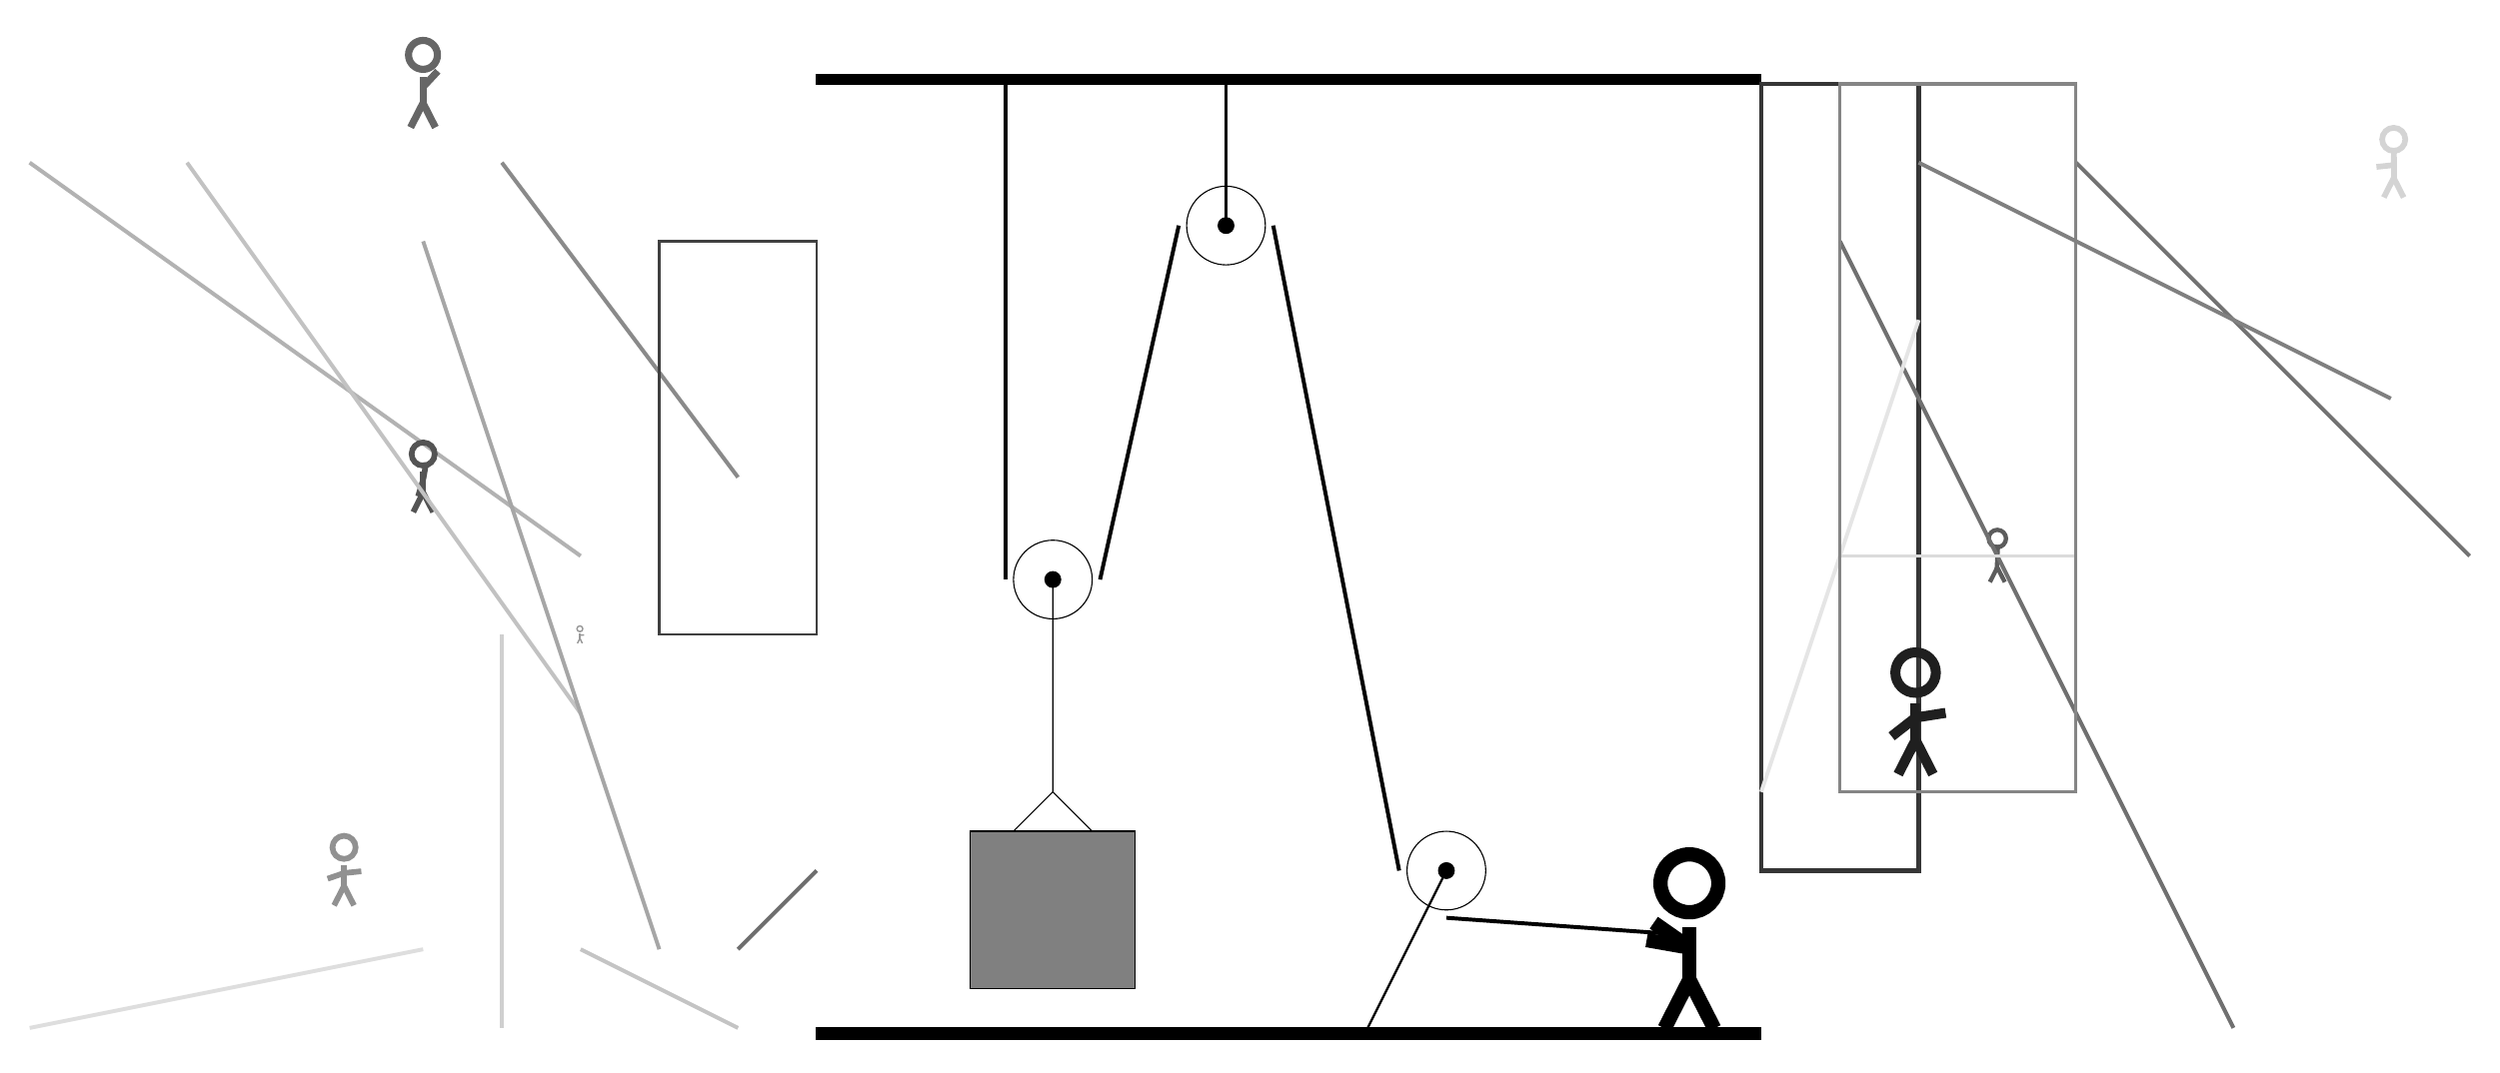
\begin{tikzpicture}
			%%%%% START %%%%%
			
			\draw[fill=black] (-2, 9) rectangle (10, 9.125);
			
			\draw[line width=0.6mm, color=black!79] (10, -1) rectangle (12, 9);
			
			\draw[line width=0.5mm, color=black!57](-3, -2) -- (-2, -1);
			\node[line width=0.5mm, color=black!17] at (18, 8) {\Strichmaxerl[4][6][89]};
			\node[line width=0.7mm, color=black!64] at (13, 3) {\Strichmaxerl[3][87][87]};
			\node[line width=0.2mm, color=black!60] at (-7, 9) {\Strichmaxerl[5][90][47]};
			\draw[line width=0.5mm, color=black!56](11, 7) -- (16, -3);
			\draw[line width=0.5mm, color=black!30](-5, 3) -- (-12, 8);
			\node[line width=0.6mm, color=black!88] at (12, 1) {\Strichmaxerl[7][38][9]};
			\draw[line width=0.5mm, color=black!19](-6, -3) -- (-6, 2);
			
			\draw[line width=0.5mm, color=black!10](12, 6) -- (10, 0);
			\draw[line width=0.5mm, color=black!55](14, 8) -- (19, 3);
			
			\node[line width=0.6mm, color=black!43] at (-8, -1) {\Strichmaxerl[4][19][6]};
			\draw[line width=0.5mm, color=black!46](-6, 8) -- (-3, 4);
			\draw[line width=0.3mm, color=black!75] (-2, 7) rectangle (-4, 2);
			\node[line width=0.6mm, color=black!67] at (-7, 4) {\Strichmaxerl[4][73][80]};
			\draw[line width=0.5mm, color=black!23](-5, -2) -- (-3, -3);
			\draw[line width=0.5mm, color=black!24](-5, 1) -- (-10, 8);
			\draw[line width=0.4mm, color=black!14] (11, 3) rectangle (14, 0);
			\draw[line width=0.4mm, color=black!48] (11, 9) rectangle (14, 0);
			
			\draw[line width=0.5mm, color=black!50](12, 8) -- (18, 5);
			\node[line width=0.4mm, color=black!40] at (-5, 2) {\Strichmaxerl[1][85][2]};
			\draw[line width=0.5mm, color=black!35](-4, -2) -- (-7, 7);
			\draw[line width=0.5mm, color=black!13](-7, -2) -- (-12, -3);
			
			\draw (3.2, 7.2) circle (0.5);
			\draw[fill=black] (3.2, 7.2) circle (0.1);
			\draw[thick] (3.2, 7.2) -- (3.2, 9);
			
			\draw (6, -1) circle (0.5);
			\draw[fill=black] (6, -1) circle (0.1);
			\draw[thick] (6, -1) -- (5, -3);
			
			\draw (1, 2.7) circle (0.5);
			\draw[fill=black] (1, 2.7) circle (0.1);
			
			\draw (1, 2.7) -- (1, 0) -- (0.5, -0.5);
			\draw (1, 0) -- (1.5, -0.5);
			\draw[fill=black!50] (-0.05, -0.5) rectangle (2.05, -2.5);
			
			\draw[line width=0.5mm] (0.4, 9) -- (0.4, 2.7);
			\centerarc[line width=0.5mm](1, 2.7)(180:360:0.6);
			\draw[line width=0.5mm](1.6, 2.7) -- (2.6, 7.2);
			\centerarc[line width=0.5mm](3.2, 7.2)(0:180:0.6);
			\draw[line width=0.5mm](3.8, 7.2) -- (5.4, -1);
			\centerarc[line width=0.5mm](6, -1)(180:270:0.6);
			\draw[line width=0.5mm](6, -1.6) -- (8.8, -1.8);
			
			\node at (9, -1.9) {\Strichmaxerl[10][-35][170]};
			
			\draw[fill=black] (-2, -3) rectangle (10, -3.15);
			
			%%%%% END %%%%%
		\end{tikzpicture}
	\end{figure}	
\end{document}